\documentclass[titlepage]{article}

\usepackage[margin=1in]{geometry}
% some more shit for the title
\usepackage[T1]{fontenc}
\usepackage{babel}

% Tables and stopping them from displaying in a different section
\usepackage{booktabs}
\usepackage[section]{placeins}

% for inserting images into the document, setting file path, and allowing rotation of inserted images 
\usepackage{graphicx}
\graphicspath{ {./images/} }
\usepackage{rotating}
\usepackage[table]{xcolor}
% mostly just for putting text in math equations
\usepackage{amsmath}
% for aligning the text to the left
\usepackage[document]{ragged2e}

% for inserting hyperlinks in the document, use \url{url} or \href{url}{text}
\usepackage{hyperref}
\usepackage{calligra}
\usepackage[T1]{fontenc}
\usepackage{siunitx}
\usepackage{caption}
\usepackage{multirow}
\usepackage[export]{adjustbox}
\usepackage{tikz}
\usepackage{pgfplots}
\pgfplotsset{soldot/.style={color=black,only marks,mark=*},
	             holdot/.style={color=black,fill=white,only marks,mark=*},
		                  compat=1.12}
\usepackage{paracol}
\usepackage{bm}

\begin{document}
\title{\textbf{Lab 3: Capacitors in Series and Parallel}}
\author{
    Zachary Pouska\\
    \texttt{001103193}\\
    \and
    Natalie Tran \\ 
    \texttt{000698629}\\ \\
} 

\date{PHYS 236 | Fall 2022\\
Date performed: 09/28/2022}


	\maketitle



	\section{Purpose}
    The purpose of this lab is to gain a working understanding of the real-world behavior of capacitors, and experimentally finding the equivalent capacitance of various combinations of series and parallel capacitors.

	\section{Theory}	

    The following formula for percent difference was used throughout the lab: $$\text{\% difference} = \frac{|C_{eq}\text{measured} - C_{eq}\text{calculated} |}{\frac{1}{2} |C_{eq}\text{measured} + C_{eq}\text{calculated}|} \times 100$$

    Equivalent capacitance is calculated using: 
    $$\frac{1}{C_{eq}} = \frac{1}{C_1}+\frac{1}{C_2} + \frac{1}{C_3}
    $$




	\section{Experiment Analysis}
    Capacitance changes with the type and amount of dielectric between the two plates. As a result of the capacitors in this lab being somewhat aged, the dielectrics inside have warped and changed shape slightly. Consequently, the capacitance in our capacitors were slightly higher than the rated values. The equation we can use to estimate some of this is given by: $$ C=\kappa \frac{\epsilon _0 A}{d}$$
    As the distance between plates decreases with warping and slow chemical reactions, the capacitance increases.

    



	\section{Procedure}

        \subsection{Measurement of Capacitance Using a Multi-Meter}
        Not using the breadboard to hold the capacitors in place, our group measured the capacitance of each capacitor while laying on the table. We then proceeded to fill out the values and calculate the percent errors in table 5.1.

        \subsection{Measurement of Equivalent Capacitance in Series}
        Beginning by assembling the capacitor circuit with backwards polarity to the example photo, our group proceeded to calculate and measure the values in table 5.2.\\ 

        \begin{figure}[hbt!] 
            \centering
            \caption*{Part 2 Circuit Diagram}
            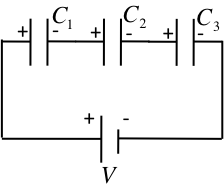
\includegraphics{images/procedure/part2.png}
        \end{figure} 

        \subsection{Measurement of Equivalent Capacitance in Parallel}
        After assembling the capacitors in parallel as shown in the figure below, our group measured the equivalent capacitance and calculated the percent difference shown in table 5.2.

        \begin{figure}[hbt!] 
            \centering
            \caption*{Part 3 Circuit Diagram}
            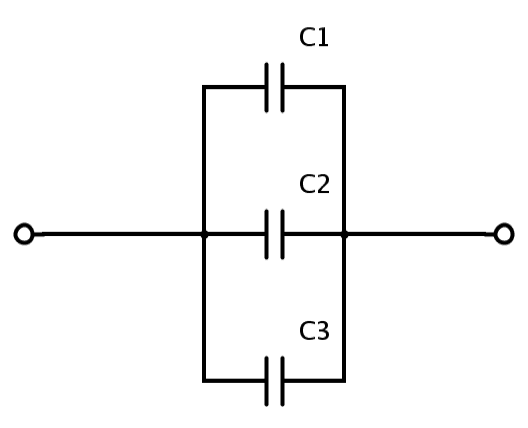
\includegraphics[scale=0.5]{images/procedure/part3.png}
        \end{figure} 



        \FloatBarrier
        \subsection{Measurement of Equivalent Capacitance for Both Series and Parallel}
        After assembling the capacitors in both parallel and series as shown below, our group measured the equivalent capacitance and calculated the percent difference shown in table 5.2.

        \begin{figure}[hbt!] 
            \centering
            \caption*{Part 4 Circuit Diagram}
            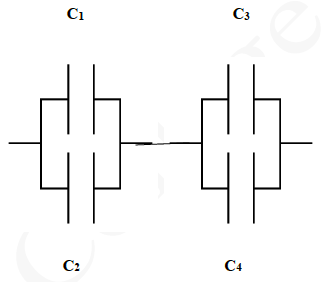
\includegraphics[scale=0.7]{images/procedure/part4.png}
        \end{figure} 


        \subsection{Measurement of equivalent capacitance for Different Configuration of Both Series and Parallel}

        \begin{figure}[hbt!] 
            \centering
            \caption*{Part 5 Circuit Diagram}
            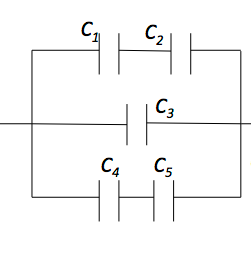
\includegraphics[scale=0.8]{images/procedure/part5.png}
        \end{figure} 
        

        \subsection{Connecting parallel capacitors to the power supply} 
        We began this experiment by discharging the capacitors, and setting up the capacitors in the configuration below. Then we collected the potential differences listed in Table 5.3. 


        \begin{figure}[hbt!] 
            \centering
            \caption*{Part 6 Circuit Diagram}
            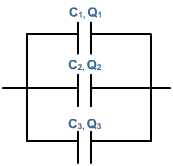
\includegraphics[scale=1]{images/procedure/part6.png}
        \end{figure} 




	\section{Data and Graphs}
	    \subsection{Part 1}
        \FloatBarrier
		\begin{table}[hbt!]
			\centering
			\rowcolors{3}{gray!10}{gray!30}
			\caption*{[\textbf{Table 5.1}] Stated Value Versus Actual Value of Capacitors}
			\begin{tabular}{c|c|c|c}
				&\textbf{Stated Value of} &\textbf{Experimental} &\textbf{Percent}\\
				& \textbf{Capacitance} & \textbf{Value Measured} & \textbf{Error}\\
				\hline
			$C_1$ & 5$\mu F$ & 5.62$\mu F$ & 12.4\% \\ 
			$C_2$ & 8$\mu F$ & 9.96$\mu F$ & 24.5\% \\ 
			$C_3$ & 10$\mu F$ & 11.2$\mu F$ & 12\% \\ 
			$C_4$ & 15$\mu F$ & 16.8$\mu F$ & 12\% \\ 
			$C_5$ & 25$\mu F$ & 28.6$\mu F$ & 14.4\% \\ 
			\end{tabular}
		\end{table}
        \FloatBarrier

	    \subsection{Part 2-5} 
		\begin{table}[hbt!]
			\centering
			\rowcolors{2}{gray!10}{gray!30}
			\begin{tabular}{c|c|c|c}
				& $\bm{C_{eq(measured)}}$ & $\bm{C_{eq(calculated)}}$ & \textbf{Percent Error} \\
				\hline
				\textbf{Part 2} &2.71$\mu F$ &2.72$\mu F$ &0.37\% \\
				\textbf{Part 3} &26.8$\mu F$ &26.78$\mu F$ &0.075\% \\
				\textbf{Part 4} &10.87$\mu F$ &10.89$\mu F$ &0.184\% \\
				\textbf{Part 5} &21.4$\mu F$ &21.38$\mu F$ &0.093\% 
			\end{tabular}
		\end{table}

	    \subsection{Part 6}
        \FloatBarrier
		\begin{table}[hbt!]
			\centering
			\rowcolors{3}{gray!10}{gray!30}
			\begin{tabular}{c|c|c|c|c}
				& Nominal Capacitance & Measured & Charge & Electric Potential\\
				& Value & Voltage &($\mu C$)) & Energy($\mu J$)\\
				\hline
			$C_1$ & 5$\mu F$ & 3.967V& 19.8 & 39.3 \\ 
			$C_2$ & 10$\mu F$ & 3.968V& 39.7 & 78.7 \\ 
			$C_3$ & 8$\mu F$ & 3.967& 31.7 & 62.9\\ 

			\end{tabular}
	   	\end{table} 
        \FloatBarrier



    \section{Calculations and Results}




	\section{Questions}


    	\subsection{Circuit 1}

        \FloatBarrier
        \begin{figure}[hbt!]
            \centering
            \caption{Circuit diagram for question 1}
            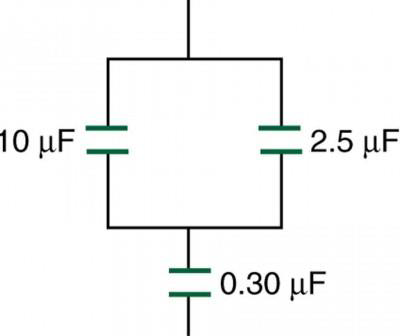
\includegraphics{questions/1}
        \end{figure}
        \FloatBarrier



    
    	\subsection{Circuit 2}
        \FloatBarrier
        \begin{figure}[hbt!]
            \centering
            \caption{Circuit diagram for question 2}
            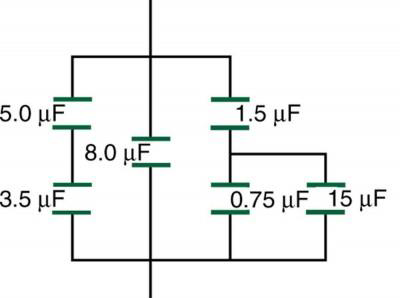
\includegraphics{questions/2}
        \end{figure}
        \FloatBarrier

    {{Calculations for finding $\mathbf{C_{eq}}$}}
        $$\left( \frac{1}{0.75\mu F+15\mu F}+\frac{1}{1.5\mu F} \right)^{-1}+\left(\frac{1}{3.5\mu F}+\frac{1}{5\mu F}\right)^{-1}+8\mu F  = 11.4 \mu F$$


    
    
  	\section{Conclusion}
    Throughout this experiment, our group measured the equivalent capacitances of various configurations of capacitors, as well as voltages in the final part, to verify the theoretical models developed throughout the previous weeks of this course. Our group was able to verify our calculations with very low percent differences, aside from the capacitors initially being quite off from their rated capacitances. It would be interesting to see how the capacitances of these capacitors change over more time as they degrade.

\end{document}
